\documentclass{standalone}
\usepackage{pgfplots} % Include package for TikZ and PGF plot
\usepackage{anyfontsize} % enable to change the font size manually 
\usepackage{makecell}%
\usetikzlibrary{shapes.geometric}
\tikzset{
dot/.style = {circle, fill, minimum size=#1,
              inner sep=0pt, outer sep=0pt},
dot/.default = 6pt % size of the circle diameter 
}
 \renewcommand{\familydefault}{\sfdefault}

\begin{document}
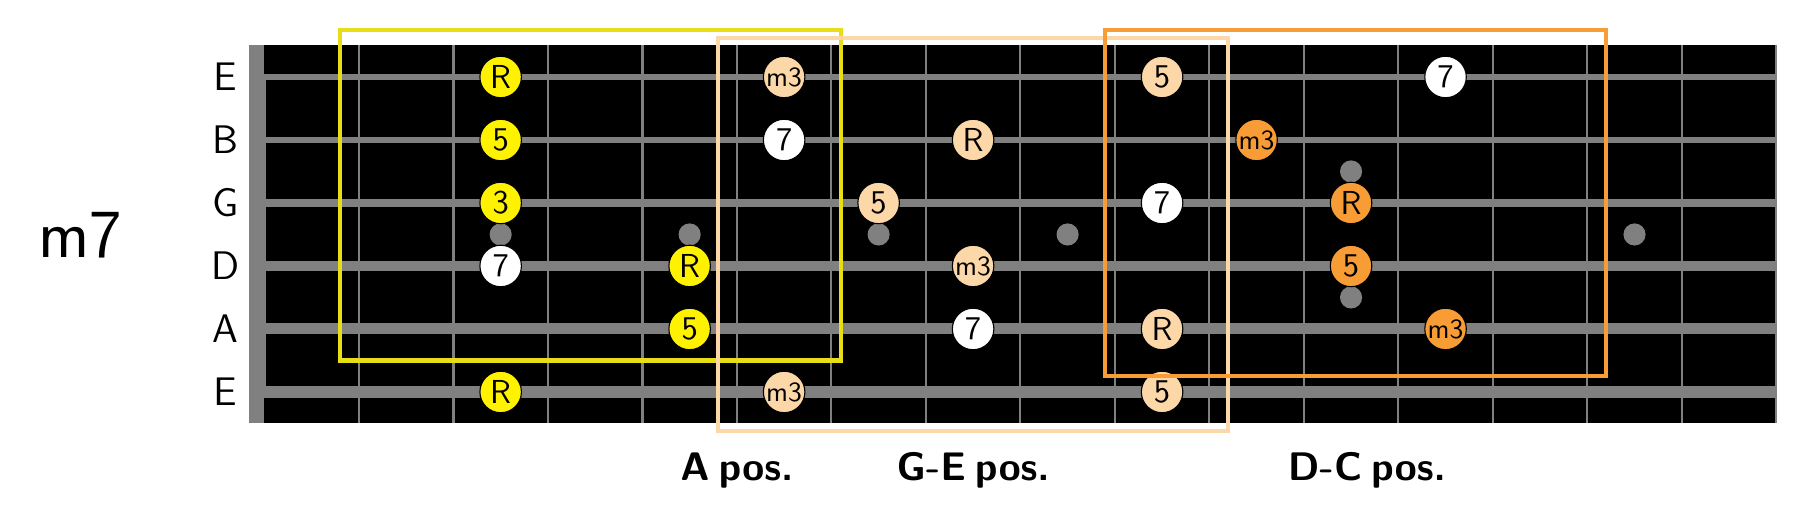
\begin{tikzpicture}[scale=1]
	\def \h{0.8}
	\def \fret{1.2} % 1.6
	\def \L{ 16*\fret }	
	\def \dot_size{4pt}
	\def \circ_size{15pt}
	
	\fill[black, line width=2] (0.0,-0.4) rectangle (16*\fret,4.4);
	\fill[black!50!white, line width=2] (-0.2,-0.4) rectangle (0,4.4);
	
	% Strings
	\draw[color=black!50!white, line width=2.0]  (-0.1, 5*\h) -- (\L,5*\h); % E
	\draw[color=black!50!white, line width=2.5]  (-0.1, 4*\h) -- (\L,4*\h); % B
	\draw[color=black!50!white, line width=3.0]  (-0.1, 3*\h) -- (\L,3*\h); % G
	\draw[color=black!50!white, line width=3.5]  (-0.1, 2*\h) -- (\L,2*\h); % D
	\draw[color=black!50!white, line width=4.0]  (-0.1, 1*\h) -- (\L,1*\h); % A
	\draw[color=black!50!white, line width=4.5]  (-0.1, 0*\h) -- (\L,0*\h); % E
	
	% Frets 0
	\draw[color=black!50!white, thick]  (-0.1, 0) -- (-0.1,5*\h); 
	\draw[color=black!50!white, thick]  (0, 0)   -- (0,5*\h); 
	
	% Fret 1-15
	\draw[color=black!50!white, thick]  (\fret,   -0.4)   -- (\fret,4.4);   
	\draw[color=black!50!white, thick]  (2*\fret, -0.4) -- (2*\fret,4.4); 
	\draw[color=black!50!white, thick]  (3*\fret, -0.4) -- (3*\fret,4.4); 
	\draw[color=black!50!white, thick]  (4*\fret, -0.4) -- (4*\fret,4.4); 
	\draw[color=black!50!white, thick]  (5*\fret, -0.4) -- (5*\fret,4.4); 
	\draw[color=black!50!white, thick]  (6*\fret, -0.4) -- (6*\fret,4.4); 
	\draw[color=black!50!white, thick]  (7*\fret, -0.4) -- (7*\fret,4.4); 
	\draw[color=black!50!white, thick]  (8*\fret, -0.4) -- (8*\fret,4.4); 
	\draw[color=black!50!white, thick]  (9*\fret, -0.4) -- (9*\fret,4.4); 
	\draw[color=black!50!white, thick]  (10*\fret, -0.4) -- (10*\fret,4.4); 
	\draw[color=black!50!white, thick]  (11*\fret, -0.4) -- (11*\fret,4.4); 
	\draw[color=black!50!white, thick]  (12*\fret, -0.4) -- (12*\fret,4.4); 
	\draw[color=black!50!white, thick]  (13*\fret, -0.4) -- (13*\fret,4.4); 
	\draw[color=black!50!white, thick]  (14*\fret, -0.4) -- (14*\fret,4.4); 
	\draw[color=black!50!white, thick]  (15*\fret, -0.4) -- (15*\fret,4.4); 
	\draw[color=black!50!white, thick]  (16*\fret, -0.4) -- (16*\fret,4.4); 
	%\draw[color=black!50!white, thick]  (17*\fret, -0.4) -- (17*\fret,4.4); 
	%\draw[color=black!50!white, thick]  (18*\fret, -0.4) -- (18*\fret,4.4); 
	%\draw[color=black!50!white, thick]  (19*\fret, -0.4) -- (19*\fret,4.4); 
	%\draw[color=black!50!white, thick]  (20*\fret, -0.4) -- (20*\fret,4.4); 
	
	% Dots
	\fill[black!50!white] (2.5*\fret,2.5*\h) circle (\dot_size); % fret 3
	\fill[black!50!white] (4.5*\fret,2.5*\h) circle (\dot_size); % fret 5
	\fill[black!50!white] (6.5*\fret,2.5*\h) circle (\dot_size); % fret 7
	\fill[black!50!white] (8.5*\fret,2.5*\h) circle (\dot_size); % fret 9
	\fill[black!50!white] (11.5*\fret,1.5*\h) circle (\dot_size); % fret 12
	\fill[black!50!white] (11.5*\fret,3.5*\h) circle (\dot_size); % fret 12
	\fill[black!50!white] (14.5*\fret,2.5*\h) circle (\dot_size); % fret 15
	%\fill[black!50!white] (16.5*\fret,2.5*\h) circle (\dot_size); % fret 17
	%\fill[black!50!white] (18.5*\fret,2.5*\h) circle (\dot_size); % fret 19
	
	% String names
	\draw[black] (-0.5,5*\h) node { {\Large E} };
	\draw[black] (-0.5,4*\h) node { {\Large B} };
	\draw[black] (-0.5,3*\h) node { {\Large G} };
	\draw[black] (-0.5,2*\h) node { {\Large D} };
	\draw[black] (-0.5,1*\h) node { {\Large A} };
	\draw[black] (-0.5,0*\h) node { {\Large E} };
	
	% Arpege (position A)
	\node[dot=\circ_size, fill=yellow,draw] at (2.5*\fret,0) {{\large R}};
	
	%\node[dot=\circ_size, fill=yellow,draw] at (0.5*\fret,1*\h) {{\large 3}};
	\node[dot=\circ_size, fill=yellow,draw] at (4.5*\fret,1*\h) {{\large 5}};
	\node[dot=\circ_size, fill=white,draw] at (2.5*\fret,2*\h) {{\large 7}};
	\node[dot=\circ_size, fill=yellow,draw] at (4.5*\fret,2*\h) {{\large R}};
	\node[dot=\circ_size, fill=yellow,draw] at (2.5*\fret,3*\h) {{\large 3}};
	\node[dot=\circ_size, fill=yellow,draw] at (2.5*\fret,4*\h) {{\large 5}};
	%\node[dot=\circ_size, fill=yellow,draw] at (0.5*\fret,5*\h) {{\large 7}};
	\node[dot=\circ_size, fill=yellow,draw] at (2.5*\fret,5*\h) {{\large R}};
	
	% Arpege (position G-E)
	\node[dot=\circ_size, fill=yellow!50!red!30!white,draw] at (5.5*\fret,0*\h) {{\normalsize m3}};
	\node[dot=\circ_size, fill=yellow!50!red!30!white,draw] at (9.5*\fret,0*\h) {{\large 5}};
	\node[dot=\circ_size, fill=white,draw] at (7.5*\fret,1*\h) {{\large 7}};
	\node[dot=\circ_size, fill=yellow!50!red!30!white,draw] at (9.5*\fret,1*\h) {{\large R}};
	\node[dot=\circ_size, fill=yellow!50!red!30!white,draw] at (7.5*\fret,2*\h) {{\normalsize m3}};
	\node[dot=\circ_size, fill=yellow!50!red!30!white,draw] at (6.5*\fret,3*\h) {{\large 5}};
	\node[dot=\circ_size, fill=white,draw] at (5.5*\fret,4*\h) {{\large 7}};
	\node[dot=\circ_size, fill=yellow!50!red!30!white,draw] at (7.5*\fret,4*\h) {{\large R}};
	\node[dot=\circ_size, fill=yellow!50!red!30!white,draw] at (5.5*\fret,5*\h) {{\normalsize m3}};
	\node[dot=\circ_size, fill=yellow!50!red!30!white,draw] at (9.5*\fret,5*\h) {{\large 5}};
	
	% Arpege (position D-C)
	\node[dot=\circ_size, fill=yellow!50!red!80!white,draw] at (12.5*\fret,1*\h) {{\normalsize m3}};	
	\node[dot=\circ_size, fill=yellow!50!red!80!white,draw] at (11.5*\fret,2*\h) {{\large 5}};	
	\node[dot=\circ_size, fill=white,draw] at (9.5*\fret,3*\h) {{\large 7}};
	\node[dot=\circ_size, fill=yellow!50!red!80!white,draw] at (11.5*\fret,3*\h) {{\large R}};
	\node[dot=\circ_size, fill=yellow!50!red!80!white,draw] at (10.5*\fret,4*\h) {{\normalsize m3}};	
	\node[dot=\circ_size, fill=white,draw] at (12.5*\fret,5*\h) {{\large 7}};	
	
	% Anotation (positions)
	\draw[black,anchor=center, text width=3.5cm, align=center] (6,-1) node { {\Large \textbf{A pos.} }};
	\draw[black,anchor=center, text width=3.5cm, align=center] (9,-1) node { {\Large \textbf{G-E pos.} }};
	\draw[black,anchor=center, text width=3.5cm, align=center] (14,-1) node { {\Large \textbf{D-C pos.} }};
	
	% Rectangle
	\draw [draw=yellow!90!black, line width=1.5] (0.8*\fret,0.4) rectangle (6.1*\fret,4.6);
	\draw [draw=yellow!50!red!30!white, line width=1.5] (4.8*\fret,-0.5) rectangle (10.2*\fret,4.5);
	\draw [draw=yellow!50!red!80!white, line width=1.5] (8.9*\fret,+0.2) rectangle (14.2*\fret,4.6);
	
	% Annotation
	\draw[black,anchor=west] (-3cm,2cm) node { {\Huge m7 } };
	
\end{tikzpicture}
\end{document}




